\documentclass[a4paper,12pt]{article}

\usepackage[czech,english]{babel}
% Fonts %
\usepackage{fouriernc}
\usepackage[T1]{fontenc}

% Colors %
\usepackage[dvipsnames]{color}
\usepackage{xcolor}

% Page Layout %
\usepackage[margin=1in]{geometry}

% Fancy Headers %
\usepackage{fancyhdr}
\fancyhf{}
\cfoot{\thepage}
\rhead{}
\renewcommand{\headrulewidth}{0pt}
\setlength{\headheight}{16pt}

% Math
\usepackage{mathtools}
\usepackage{amssymb}
\usepackage{faktor}
\usepackage{import}
\usepackage{caption}
\usepackage{subcaption}
\usepackage{wrapfig}
\usepackage{enumitem}
\usepackage{tikz}
\usetikzlibrary{cd,positioning,babel,shapes}
\usepackage{tkz-base}
\usepackage{tkz-euclide}

% Theorems
\usepackage{amsthm}
\usepackage{thmtools}

% Title %
\title{\Huge\textsf{Linear Equations}\\
 \Large\textsf{Scales, Lines \& Functions}
 \author{Áďa Klepáčů}
 \date{\today}
}

% Table of Contents %
\usepackage{hyperref}
\hypersetup{
 colorlinks=true,
 linktoc=all,
 linkcolor=blue
}

% Tables %
\usepackage{booktabs}
\usepackage{tabularx}

% Patch for hyphens
\usepackage{regexpatch}
\makeatletter
% Change the `-` delimiter to an active character
\xpatchparametertext\@@@cmidrule{-}{\cA-}{}{}
\xpatchparametertext\@cline{-}{\cA-}{}{}
\makeatother

\newcolumntype{s}{>{\centering\arraybackslash}p{.4\textwidth}}

% Operators %
\DeclareMathOperator{\Ker}{Ker}
\DeclareMathOperator{\Img}{Im}
\DeclareMathOperator{\End}{End}
\DeclareMathOperator{\Aut}{Aut}
\DeclareMathOperator{\Inn}{Inn}

% Common operators %
\newcommand{\R}{\mathbb{R}}
\newcommand{\N}{\mathbb{N}}
\newcommand{\Z}{\mathbb{Z}}
\newcommand{\Q}{\mathbb{Q}}
\newcommand{\C}{\mathbb{C}}

\newcommand{\tr}{\textcolor{red}}
\newcommand{\tb}{\textcolor{blue}}
\newcommand{\tg}{\textcolor{green}}
\newcommand{\tm}{\textcolor{magenta}}
\newcommand{\tv}{\textcolor{violet}}

% American Paragraph Skip %
\setlength{\parindent}{0pt}
\setlength{\parskip}{1em}

% Document %
\pagestyle{fancy}
\begin{document}

\thispagestyle{fancy}

\section*{Web -- úloha 3}

V souboru \texttt{app.py} máte připravenou aplikaci ve Flasku a ve složce
\texttt{templates} její šablony. Máte za úkol dvě věci:
\begin{itemize}[topsep=0pt]
 \item Zařídit, aby odkaz \uv{Stránka 1} v šabloně \texttt{home\_page.html} vedl
  na umístění (path) \texttt{/page1}.
 \item Na tomto umístění (\texttt{/page1}) přes funkci \texttt{page1} v
  \texttt{app.py} vykreslit šablonu \texttt{page1.html} a vypsat v ní obsah
  seznamu \texttt{items} v tagu \texttt{ul}.
\end{itemize}
Aplikaci můžete ve VSCodu spustit tak, že ho otevřete ve složce se zadáním a v
terminálu (horní lišta $ \to $ \texttt{Terminal}) zadáte \texttt{flask run
---debug}.
\begin{center}
 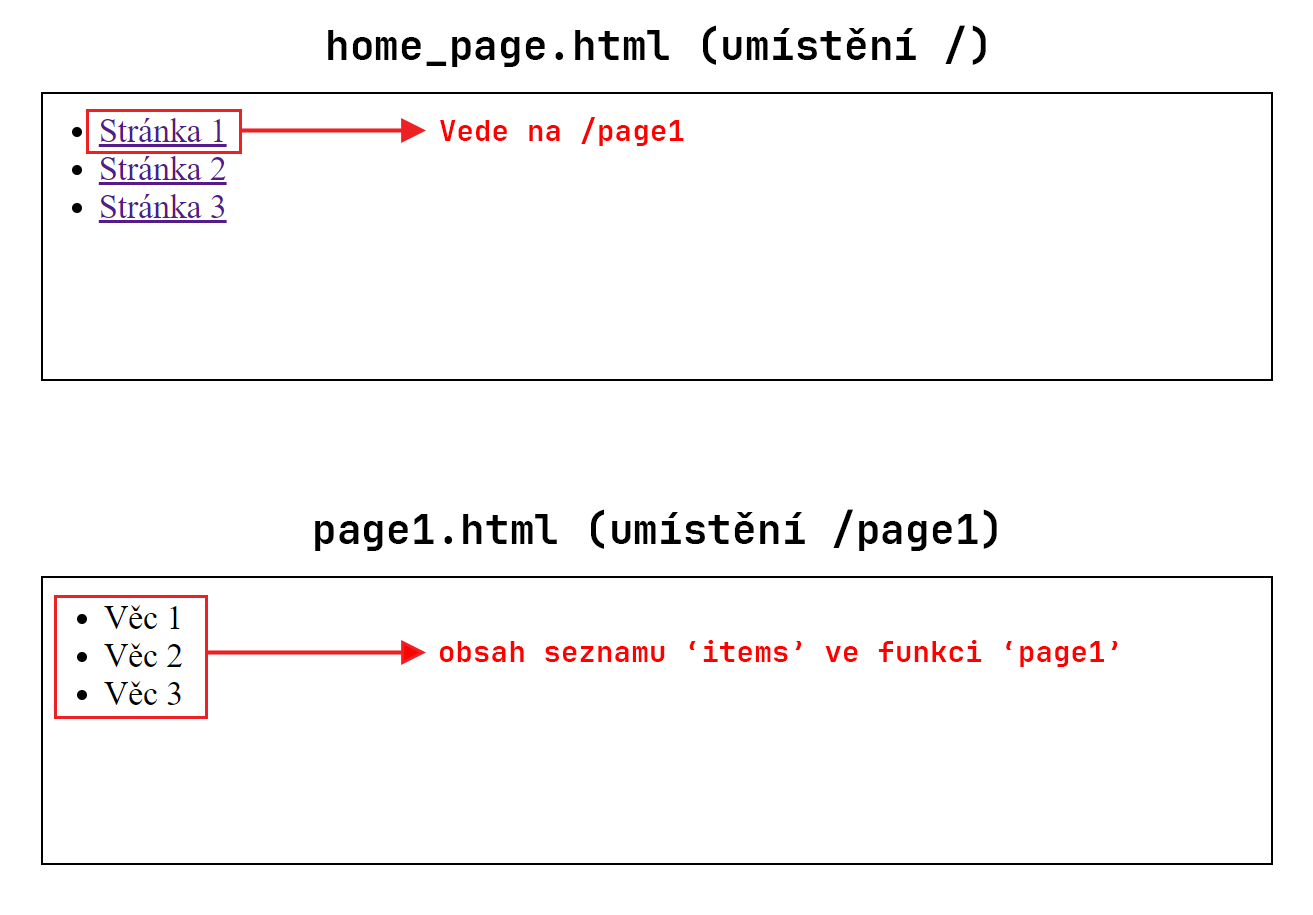
\includegraphics[width=\textwidth]{pomucka.png}
\end{center}
\end{document}
